\chapter{Simon's Algorithm}
\section{Problem}
In the Simon's Problem, we have a function $f$ which is one-one or two-one, i.e. the values for each input may be unique(one-one) or two inputs may the same output(two-one). Further, if the function is two-one, we have a hidden bit-string $s$ such that\begin{equation}
\text{if } f(x_1) = f(x_2) \text{ then } x_1\oplus x_2 = s
\end{equation}our objective is to find whether $f$ is one-one or in the other case, find the bit-string $s$.
\section{Classical Soution}
In the classical regime, the worst case scenario takes $2^{n-1} + 1$ calls to the function $f$ where $n$ is the number of bits required to represent the input of $f$. In the worst case, all the numbers that we sample returns different values of $f(x)$. This can happen for at max $2^{n-1}$ times. hence, we would require one more call to get the final result. 
\section{Quantum Solution}
\begin{figure}[h]
\centering
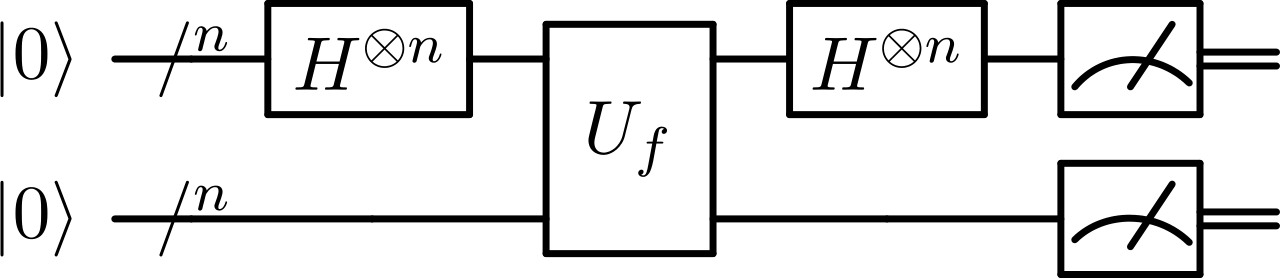
\includegraphics[width=0.7\textwidth]{images/simon.png}
\label{simon algo}
\caption{Circuit for Simon's Algorithm}
\end{figure}
The above circuit shows the circuit used to solve the Simon's Problem. The circuit is similar to the Deutsch-Josza one. Here again, $U_f$ is the quantum oracle for the function $f$. Let us see what each step does.
\begin{enumerate}
\item The initial state consist of two registers consisting of $n$ qubits. Both are initialised to $|0\rangle^{\otimes n}$ . So, $|\psi_0\rangle = |0\rangle^{\otimes n}|0\rangle^{\otimes n}$
\item First we apply Hadamard gate to the irst register. the vaue of the qubits changes to:\begin{equation}
|\psi_1\rangle = \frac{1}{\sqrt{2^{n}}}\left( \sum_{x=0}^{2^n -1} |x\rangle \right)|0\rangle^{\otimes n} 
\end{equation}
\item Then we apply the quantum oracle changing the second register to $f(x)$. The new state is \begin{equation}
|\psi_2\rangle = \frac{1}{\sqrt{2^{n}}}\left( \sum_{x=0}^{2^n -1} |x\rangle |f(x)\rangle\right)
\end{equation}
\item Applying Hadamard again, and using the general transformation for $H^{\otimes n}$,\begin{equation}
|\psi_3\rangle = \frac{1}{2^{n}} \sum_{x=0}^{2^n -1} \left(\sum_{z=0}^{2^n -1} (-1)^{x.z} |z\rangle\right)|f(x)\rangle
\end{equation}
\item Measure the two registers. The second register is measured first. When the second register is measured, the value of first register collapses to the values which have $f$ as measured with Hadamard applied on them. So, \begin{equation}
\text{For one-one, } |\psi_4\rangle =  \frac{1}{\sqrt{2^{n}}} \sum_{z=0}^{2^n -1} (-1)^{x.z} |z\rangle \\
\end{equation}\begin{equation}
\begin{split}
\text{For two-one, } |\psi_4\rangle & =  \frac{1}{\sqrt{2^{n+1}}}\left( \sum_{z=0}^{2^n -1} (-1)^{x.z} |z\rangle + \sum_{z=0}^{2^n -1} (-1)^{y.z} |z\rangle\right) \\ & = \frac{1}{\sqrt{2^{n+1}}} \sum_{z=0}^{2^n -1}\left( (-1)^{x.z} + (-1)^{y.z}\right)|z\rangle
\end{split}
\end{equation}Note that by the given condition defining s,we have $y = x \oplus s$.
\item now measure the first register. If the value is $|0\rangle^{\otimes n}$, this means that $(-1)^{x.z} = (-1)^{y.z}$. If this equality does not hold, we get some other value. Notice the condition. \begin{equation}
\begin{split}
(-1)^{x.z} &= (-1)^{y.z} \\ 
\Rightarrow x.z &= y.z \mod{2}\\
\Rightarrow x.z &= (x \oplus s).z \mod{2}\\
\Rightarrow x.z &= x.z \oplus s.z \mod{2}\\
\Rightarrow s.z &= 0 \mod{2}\\
\end{split}
\end{equation}If the above equation does not hold, then $s.z = 1 \mod{2}$.
\end{enumerate}
If we have to find $s$, we have to basically find the value of each of the bits. For this, we will need n equations as $s$ is of $n$ bits. So, repeating the above process till we get $n$ different $z$, we will get $n$ different equations and hence the value of $s$ can be determined.\\
The above algorithm needs about $O(p(n))$ runs of the above circuit, where $p(\cdot )$ is a polynomial function. Again, using quantum computer leads to an exponential speedup.

